\documentclass[10pt,a4paper,twoside]{article}

% Please make sure that spp.dat (supplied with this template) is in your working directory or path
\input{spp2024.dat}

\renewcommand{\P}[1]{\left( #1 \right)}
\renewcommand{\l}{\ell}
\renewcommand{\ref}[1]{Fig. #1}

\begin{document}
	
\title{\TitleFont Gaussian component of beams with fractional topological charge}

\author[*]{Maria Isabella M.~Mendoza~\authorsep}
\author[ ]{Nathaniel Hermosa \authorsep}
\author[ ]{Ni\~na Zambale Simon~\lastauthorsep}
\affil[ ]{National Institute of Physics, University of the Philippines Diliman, Philippines}
\affil[*]{\corremail{mmmendoza31@up.edu.ph} }
\maketitle
\thispagestyle{titlestyle}

\section*{Response to review}
	\paragraph
	~Dear Editor,
	\paragraph
	~We extend our thanks to the reviewer for their time and constructive criticism. We are now forwarding our revised manuscript (attached) with our responses and list of revisions below.
	
	\begin{enumerate}
		\item \textit{"For Figure 3 the label legend may I know if it is correct they both have the same label for integer and half integer."}
		
		We did not change these color labels --- they originally already distinguish the data at integer and half-integer $\l$ from the rest. Nevertheless, we now also changed their markers for greater emphasis.
		
		\item \textit{Please also reconsider the size of the subpanels in Figs 2-3. When printed, if they do not provide helpful information, maybe it is better to omit some panels. Please favor effectiveness over overcompleteness.}
		
		We thank the reviewer for pointing out this issue. To reduce redundancy as well, only subpanels around one example each of integer $\l$ ($\l = 1.0, 1.2$) and half-integer $\l$ ($\l = 2.4, 2.6$) were retained. However, to aid explanation in $\l \in [0, 1]$, subpanels were added in that range too. As such, the pictures are now also enlarged.
		
		Kindly find the revised Figure 3 below:
		
		\begin{figure}[h!]
			\centering
			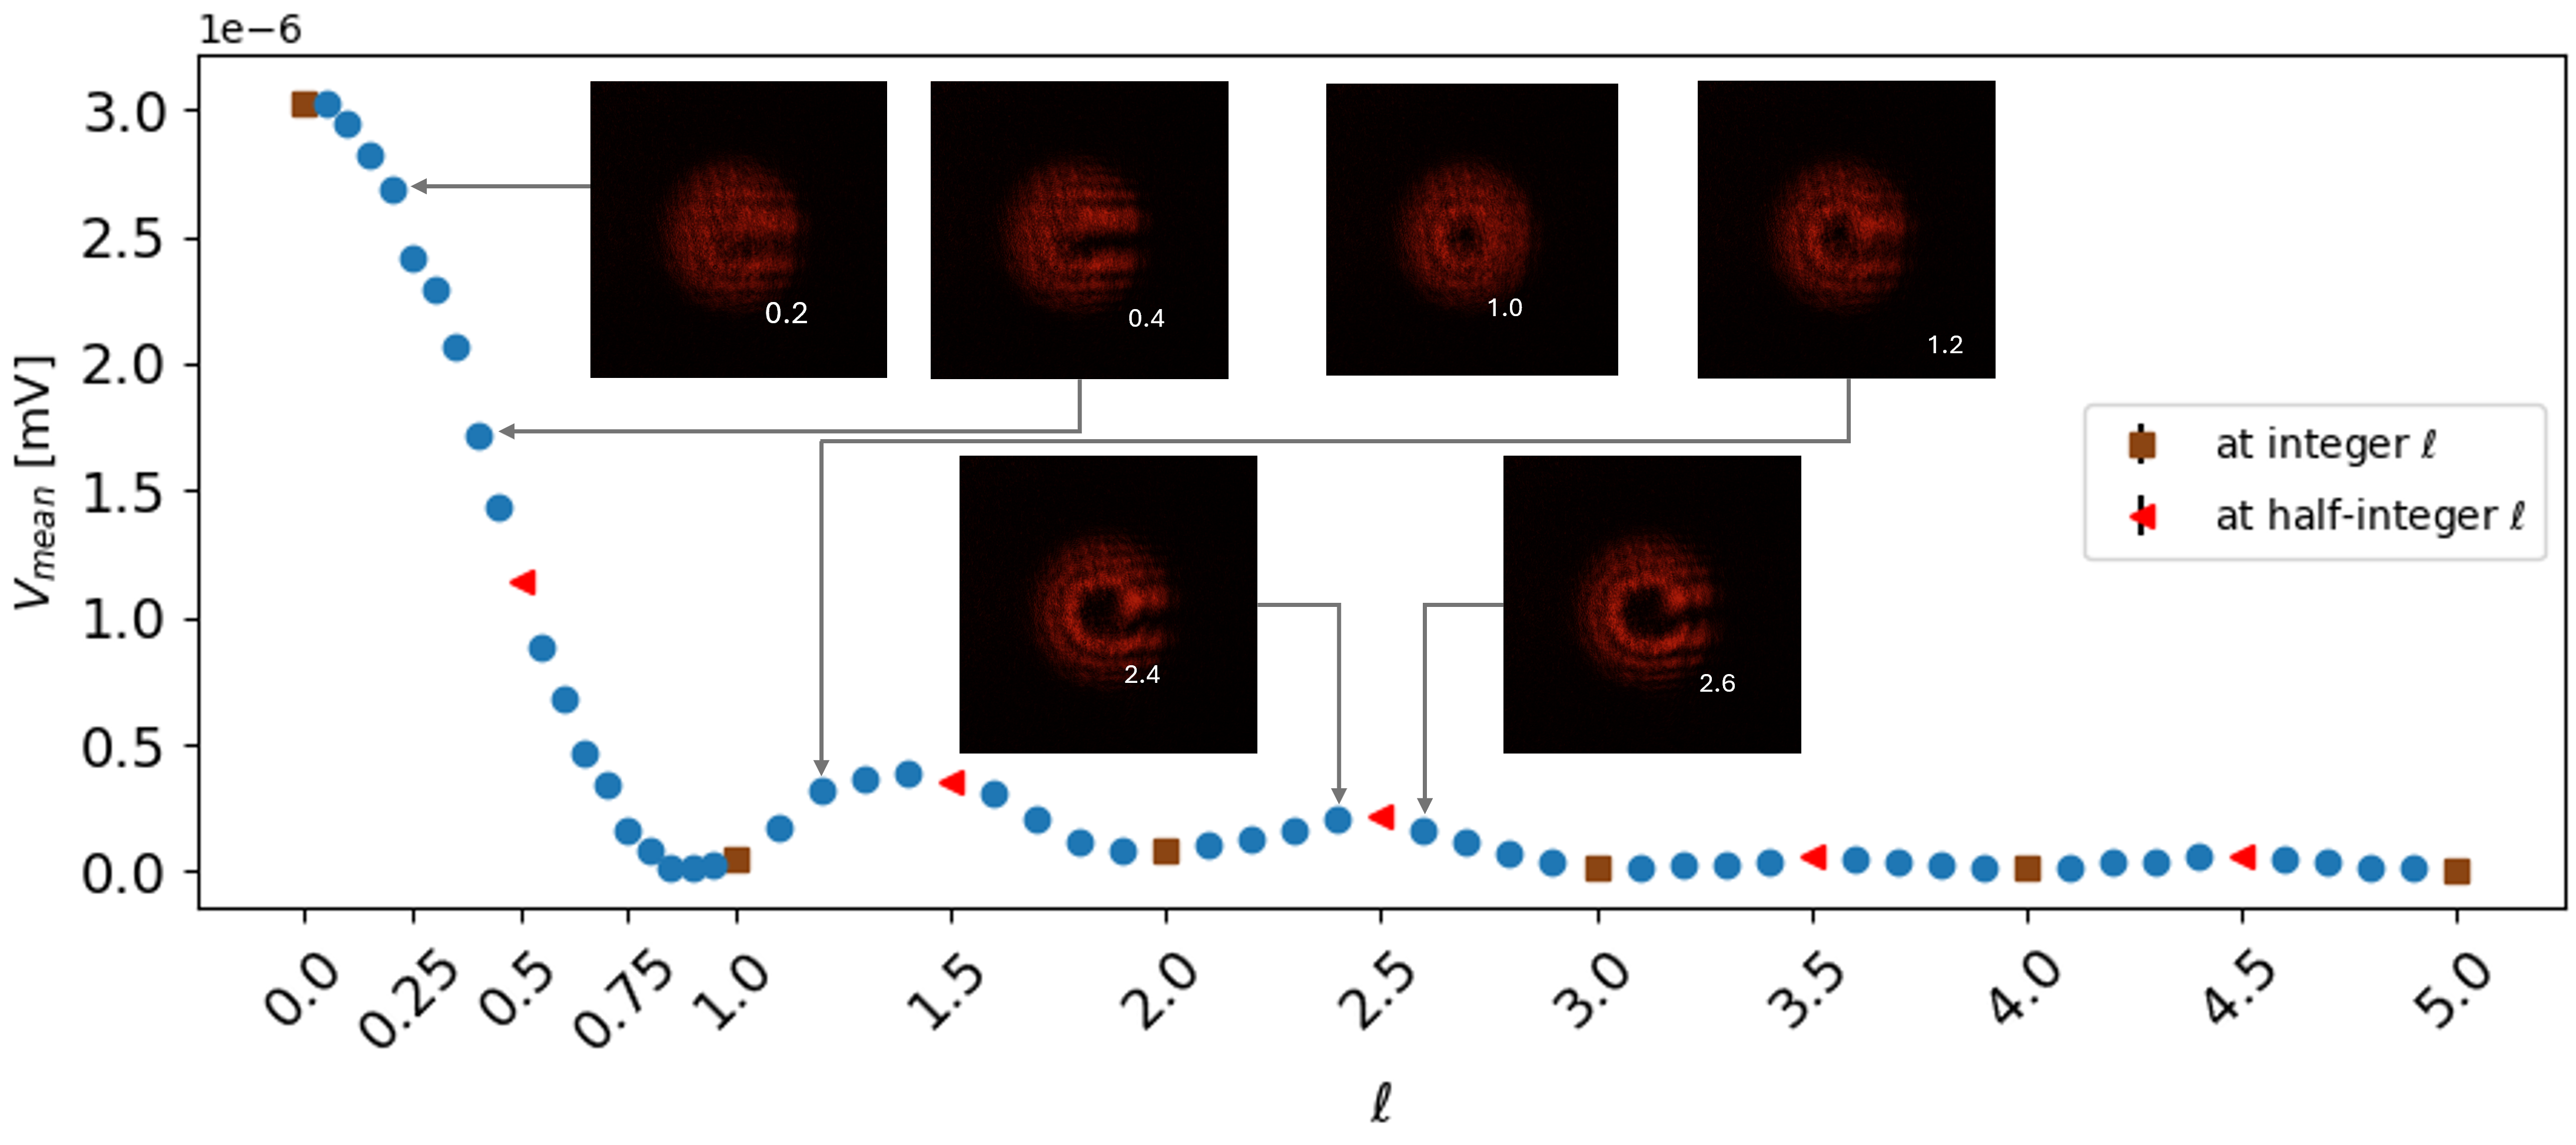
\includegraphics[width=0.85\textwidth]{SMF.png}
			\caption{[Figure 3] Mean voltage $V_{mean}$ representing the Gaussian component at each value of $\l$. The voltage curve has local peaks for half integer values of $\l$ (e.g. $\l = 1.5, 2.5$). Errorbars (black) are obscured by the markers.}\label{fig:V}
		\end{figure}
		
		\item (Editorial comment) \textit{Please make the abstract self-contained by using full citation details, eg [Phys. Rev. A YY, 1567 (2xxx)].}
		
		We have fixed the format of our only citation in the abstract.
		
		\item We have also fixed the bibliography to conform to SPP format - using the abbreviated journal name and deleting unnecessary keys. We have also fixed the double listing of a reference in the bibliography --- apologies for this oversight.
	\end{enumerate}
	

	\paragraph
	~While the reviewer's comments have been helpful for readability, we have also made some corrections and clarifications:
	
	\begin{enumerate}
		\item We now correct in the Methodology that the voltage values are gathered for \textbf{smaller interval of $\l$ (0.05) for $\l \in [0, 1]$}, as opposed to 0.1 interval for the rest of the data. In contrast, the first submission stated 0.05 interval for \textbf{all} $\l$. Moreover, it is now explained under Results and Discussion that this data acts as a sanity check that the beam is better aligned with the fiber, since fiber alignment was a major source of error in early versions of the data.
		\item In relation to that, we have now attempted to explain the monotony of the decrease in $\l \in [0,1]$.
		\item In Figure 2, the range of $\l$ for which intensity profiles were shown was corrected from $\le 5$ to $< 5$.
		%\item probably fill in literature review in the Introduction
		\item In the Introduction, we have also improved the construction of some sentences and defined variables.
		\item The GitHub repository, containing the programming scripts, has been renamed to be more descriptive of the study.
	\end{enumerate}
	
	\paragraph
	~We look forward to hearing your response on our study, as well as any further recommendations for revisions.
	
	\paragraph
	~Thank you,
	\paragraph
	~Maria Isabella M. Mendoza,
	
	Nathaniel Hermosa,
	
	Ni\~na Zambale Simon
		
\end{document}